%\section{Dynamic response of QGP to electromagnetic fields}
\subsection{Electromagnetic plasma properties of QGP}\label{chap:QCD}
%%%%%%%%%%%%%%%%%%%%%%%%%%%%%%
\para{The electromagnetic QGP medium}
{\color{black} The experimental study of QGP utilizing relativistic heavy-ion collisions provides the only known method to probe some key cosmic QGP properties. In these collisions, the strongly interacting quarks and gluons reach conditions that have governed the early Universe during its primordial quark-gluon plasma epoch, where the temperature exceeded the hadronization condition $T>150\MeV$.} 

{\color{black} Aside from strongly screened color-strong interactions, the QGP phase is governed by the electromagnetic(EM) properties of quarks. EM response of QGP is of particular interest considering possible cosmic magnetic fields that may have been generated and/or are present during the QGP epoch; we return to this topic in quantitative detail in \rsec{sec:mag:universe}. Novel EM mechanisms in QGP, such as the chiral magnetic effect \cite{Kharzeev:2007jp}, could also have an interesting impact. Long range cosmic magnetic fields could influence particle interactions and plasma dynamics, similar to how strong magnetic fields play a role in relativistic heavy-ion collisions. The transport properties, such as the electromagnetic conductivity of QGP, are essential for understanding how electromagnetic fields evolve and how particles interact within the plasma.}

{\color{black} The heavy-ion collision experiments allow us to explore how cosmic-scale magnetic fields might have affected the QGP's behavior. This insight directly connects laboratory studies to cosmological phenomena, offering a window into the Universe’s primordial state. In this section, we will review a semi-analytic study of the electromagnetic field of heavy ions in QGP following Ref.\,\cite{Grayson:2022asf}. This method may lead to the experimental determination of the electromagnetic conductivity of QGP which influences decisively the freeze-out magnetic field in heavy ion collisions~\cite{STAR:2023jdd}. This would provide the required insight into the EM properties of strongly interacting primordial QGP, such as the electric conductivity, present during the early Universe.}

{\color{black} The semi-analytic framework discussed below builds the groundwork for understanding the electromagnetic properties of QGP in heavy ion collisions allowing us to describe the strongly interacting particle plasma in the early Universe. By studying QGP experimentally in the collisions of heavy ions, we aim to determine its electromagnetic transport properties, such as its static conductivity, which can then be used to infer the properties of QGP in the early Universe.}

%%%%%%%%%%%%%%%%%%%%%%%%%%%%
\para{Transport theory methods}
We consider the ultra-relativistic limit of the polarization tensor seen in Chapter \ref{chap:PlasmaSF} to study the electromagnetic properties of quark-gluon plasma (QGP) \cite{Grayson:2022asf}. We are interested in understanding  electromagnetic fields generated by colliding relativistic heavy-ion collisions which arguably  the largest in the known Universe, on the order of 
\begin{equation}\label{eq:Bcol}
ec|B| \approx m_\pi^2,
\end{equation}
but exist for very short times 
\begin{equation}\label{eq:tcol}
t_{\text{coll}}= 2 R/\gamma \sim 10^{-25}\,\textrm{s}\,,
\end{equation}
due to the Lorentz contraction by the Lorentz-factor $\gamma$ of the colliding nuclei. The magnetic field\index{magnetic!field} generated in these collisions is interesting due to its role in separating electric charge in the QGP through the chiral magnetic effect (CME) \cite{Kharzeev:2007jp}.

The electric current generated by the CME could lead to a charge separation along magnetic field lines. If a magnetic field survives in QGP until the time of hadronization\index{QGP!hadronization} of the QGP, which we will refer to as the freeze-out time $t_f$, it could also lead to a difference in the observed global polarization of $\Lambda$ hyperons and anti-hyperons\index{hyperon} \cite{Muller:2018ibh}. Charge separation in the hadron was recently studied experimentally \cite{STAR:2023jdd}. 

The distribution of the vacuum magnetic field\index{magnetic!fields} of two colliding nuclei in the center of momentum frame (CM-frame) is given by the Li\'enard-Wiechert fields shown in \rf{fig:vacmag}. This is the same magnetic field found by Lorentz boosting the Coulomb field of a nucleus at rest. We neglect the portion of the field that depends on acceleration arising in the actual collision since it is small for in vacuum scattering of heavy nuclei, as compared to the field that depends only on velocity.

%%%%%%%%%%%%%%%%%%%%%%%%%
\begin{figure}
\centering 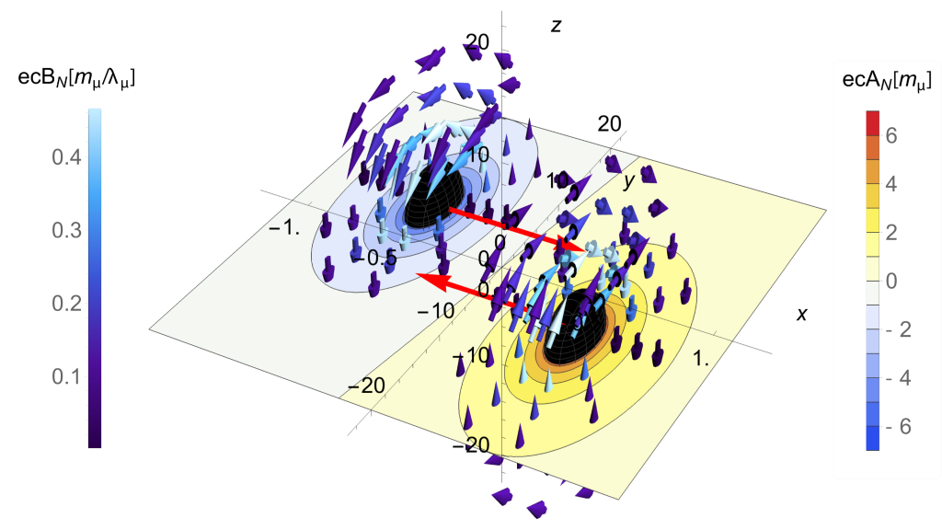
\includegraphics[width=0.85\linewidth]{plots/Bfield.png}
\caption{The vacuum magnetic field and vector potential for two colliding lead Pb nuclei. See text for further discussion. \radapt{Grayson:2024okq}.}
    \label{fig:vacmag}
\end{figure}
%%%%%%%%%%%%%%%%%%%%%%%%%%%%%%%

{\color{black}The vacuum magnetic field  and the vacuum vector potential is depicted in \rf{fig:vacmag}  for the case of two colliding lead Pb nuclei in CM-frame. The vector potential is plotted in the collision plane in the right-half of figure, the magnetic field on left-half.  Red arrows indicate the direction of the moving nuclei with an impact parameter $b=3R$, $R$ is nuclear radius, and the Lorentz-factor $\gamma =37$.  At a larger Lorentz-factor, a graphical representation is difficult to visualize without scaling the fields with $\gamma$.  This plot shows how the magnetic field distribution is Lorentz contracted along the direction of motion. The magnetic field lines circulate out of the collision plane perpendicular to the velocity, adding together at the collision center.} 

This magnetic field is treated as an external perturbation on the quark-gluon plasma, filling the overlap region between the two nuclei after they collide. For simplicity, the QGP is modeled as an infinite medium to avoid edge complications at the plasma boundary. The temperature of QGP depends strongly on the collision energy of the nuclei. In \cite{Grayson:2022asf} we study Au+Au collisions at $\sqrt{s_{\text{NN}}}=200\,$GeV for QGP temperature $T=300$\,MeV.  After Heavy Ions collide, the conducting QGP medium generates long-range decaying tails or wake-fields in the magnetic field that extend far beyond the collision time \cite{Tuchin:2010vs}. The conductivity of QGP determines the strength of these wake-fields. We aim to model these fields in QGP using the formulation discussed in Chapter \ref{chap:PlasmaSF}.

%%%%%%%%%%%%%%%%%%%%%%%%%%%%
\para{EM conductivity of quark-gluon plasma}
Past analytic calculations \cite{Tuchin:2010vs,Deng:2012pc,McLerran:2013hla,Tuchin:2013apa,Gursoy:2014aka,Li:2016tel,Roy:2015kma} solve Maxwell's equations in the presence of static electric conductivity 
\begin{equation}
   \sigma_0 = \frac{m_D^2}{3\kappa}\,,
\end{equation} 
in a  hydrodynamically evolving QGP. For a collisionless plasma $\kappa\rightarrow0$, the conductivity is infinite, and the medium behaves as a perfect conductor. Our work introduces the frequency and wave-vector dependence of the QGP analytically using the polarization tensor previously obtained in Ref.\,\cite{Formanek:2021blc}.

Prior work \cite{Inghirami:2016iru,Inghirami:2019mkc} incorporated the dynamical response of QGP by numerically solving the coupled magneto-hydrodynamic equations for a conducting quark-gluon plasma in the presence of the colliding nuclear charges. More recent calculations \cite{Yan:2021zjc,Wang:2021oqq} also incorporate the frequency and wave-vector dependence of the QGP response to electromagnetic fields by solving the coupled Vlasov-Boltzmann--Maxwell equations\index{Vlasov-Boltzmann equation}  numerically.

%%%%%%%%%%%%%%%%%%%%%%%%%%%%%
\para{The Ultrarelativistic EM polarization tensor in QGP}
Here we review the ultra-relativistic polarization tensor, including damping, for the idealized case where the QGP is infinite, homogeneous, and stationary. This calculation differs from our earlier work \cite{Formanek:2021blc} only in that we consider three quark species: up, down, and strange in thermal equilibrium abundance. We start with the Vlasov-Boltzmann equation for each quark flavor \req{eq:boltzmanncov}, where we assume all quarks collide on a momentum-averaged time scale $\tau_{\text{rel}} = \kappa^{-1}$. The induced current $ j_{\mathrm{ind}}^\mu$ can be written in terms of the phase-space distribution of quarks and anti-quarks as
\begin{equation}\label{eq:current}
   j_{\mathrm{ind}}^\mu(x) = 2 N_c \int (dp)p^\mu \\ \times \sum_{u,d,s} q_f (f_{f}(x,p) - f_{\bar{f}}(x,p))=  4 N_Q e^2 \int (dp)p^\mu \delta f(x,p)\,,
\end{equation}
where  $N_c$ is the number of colors. We sum over the quark flavors with charges $q_f$, and in the final result, we replace $q_f \delta f = \delta f_f$. The result \req{eq:current} differs from that found in the case of an electron-positron plasma by the factor
\begin{equation}
N_Q \equiv N_c\sum_f (q_f/e)^2 = 2\,,
\end{equation}
for three light quark flavors ($u,d,s$).

In the ultrarelativistic limit, neglecting quark masses, one finds the polarization functions \cite{Formanek:2021blc}:
\begin{align}\label{eq:polfuncsUltra}
&\Pi_{\parallel}(\omega,|\boldsymbol{k}|) = m_D^2\frac{\omega^2}{\boldsymbol{k}^2}\left(1 - \frac{\omega \Lambda}{2|\boldsymbol{k}|-i\kappa \Lambda}\right)\,,\\
&\Pi_{\perp}(\omega,|\boldsymbol{k}|) = \frac{m_D^2\,\omega}{4 |\boldsymbol{k}|}\left( \Lambda \left(\frac{\omega'^2}{\boldsymbol{k}^2} - 1\right) - \frac{2\omega'}{ |\boldsymbol{k}|}\right)\,,
\end{align}
where $\Lambda(\omega,\boldsymbol{k})$ is defined as
\begin{align}\label{eq:definitions}
 \Lambda \equiv \ln \frac{\omega'+  |\boldsymbol{k}|}{\omega'- |\boldsymbol{k}|}\,, \quad \text{with} \quad \omega' = \omega+i\kappa\,.
\end{align}
The parallel and transverse polarization functions have the same form as in \cite{Formanek:2021blc} except for an overall factor $N_Q$  as found in \cite{Kapusta:1992fm,Grayson:2022asf}:
\begin{equation}\label{eq:DebyemQCD}
    {m_D}^2_{(\text{EM})} = \sum_{u,d,s} q^2_f T^2 \frac{N_c}{3} = N_Q\frac{e^2T^2}{3} \equiv C_{\text{em}}T^2\,,
\end{equation}
where $C_{\text{em}} =  2e^2/3$. In the following, we will use $m_D$ as short-hand notation for the electromagnetic screening mass since we do not discuss color screening here.
The transverse conductivity $\sigma_{\perp}$, which controls the response of the plasma to magnetic fields\index{magnetic!fields}, is related to the imaginary part of the transverse polarization function as in \req{eq:sigmaperp}.

%%%%%%%%%%%%%%%%%%%%%%%%%%%%%%
\para{QCD Damping rate and simple models of conductivity in QGP}
The strength of the plasma response to an external magnetic field depends on the quark damping rate $\kappa$ and the electromagnetic screening mass $m_D$. The scale of the collisional quark damping $\kappa$ is much larger than the electromagnetic Debye mass $m_D$ and electromagnetic damping $\kappa_{\text{EM}}$ because it depends on the strong coupling constant $\alpha_s$, not the electromagnetic coupling $\alpha$.

In \cite{Grayson:2022asf}, we use the first-order electromagnetic Debye mass \req{eq:DebyemQCD} to estimate the electromagnetic screening mass $m_D$. The collision rate $\kappa$ is related to the inverse of the mean-free time of quarks in QGP. We adopt a value for $\kappa$ from \cite{Mrowczynski:1988xu} where the mean-free time is given by the product of the parton density in the QGP and the quark-parton transport cross-section, leading to the expression 
\begin{equation}\label{eq:kappadef}
    \kappa(T) = \frac{10}{17\pi} (9 N_f +16) \zeta(3) \alpha_s^2 \ln\left(\frac{1}{\alpha_s}\right) T\,,
\end{equation}
where $N_f$ is the number of flavors, $\zeta(x)$ denotes the Riemann zeta function, and $\alpha_s(T)$ is the running QCD coupling.  We model the running of the QCD coupling constant as a function of temperature in the range $T<5T_c$ using a fit provided in \cite{Letessier:2002ony}:
\begin{equation}\label{eq:alphas}
    \alpha_s(T) \approx \frac{\alpha_s(T_c)}{1+C \ln(T/T_c)}\,,
\end{equation}
where $C=0.760 \pm 0.002$. For the QCD (pseudo-)critical temperature we use $T_c = 160\,$MeV. The  electromagnetic QED Debye mass is compared to $\kappa(T)$ in \rf{fig:kappaDebye}. We  expect the electromagnetic response of QGP to be over-damped since $\kappa> \frac{2}{\sqrt{3} m_D}$ giving a plasma frequency \req{eq:plasmafreq} which is imaginary over the range of temperatures relevant for QGP. We note that at the QGP temperature $T=300\,$MeV we use as example, $\kappa = 4.86\, m_D$.    

%%%%%%%%%%%%%%%%%%%%%
\begin{figure}
    \centering
    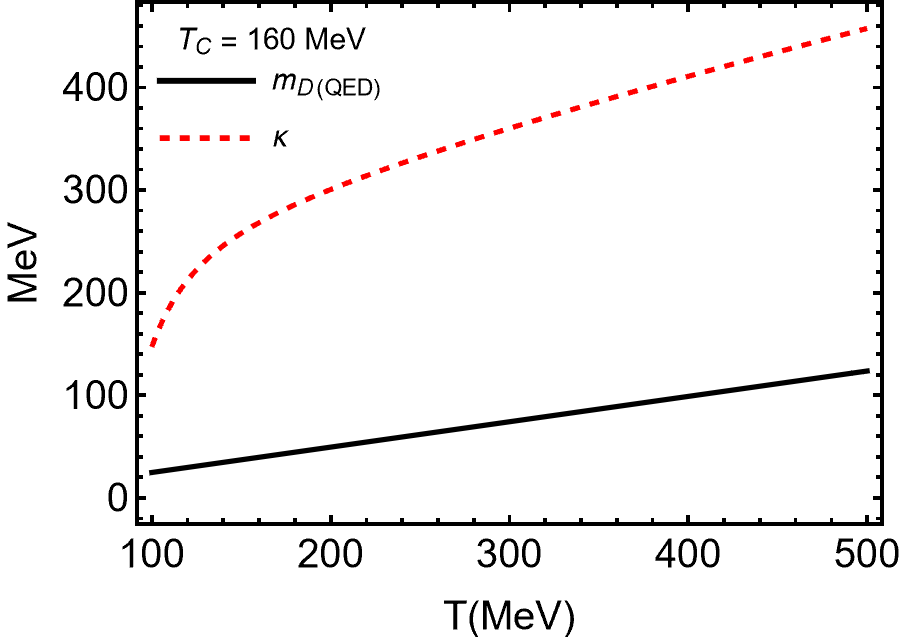
\includegraphics[width=0.7\linewidth]{plots/kappaDEBYE.png}
    \caption{The electromagnetic Debye mass $m_D$, solid (black) line, and the QCD dampening rate $\kappa$, dashed (red) line, as a function of temperature.  \cccite{Grayson:2022asf}}
    \label{fig:kappaDebye}
\end{figure}
%%%%%%%%%%%%%%%%%%%%%%%%%%%%



A  well studied model of conductivity is the Drude model~\cite{Drude:1900}, the long wavelength limit $k \to 0$ of the conductivity, which of course is isotropic as it depends only of $\omega$
\begin{equation}\label{eq:drude}
    \sigma_\parallel(\omega,0) = \sigma_\perp(\omega,0) = \frac{\sigma_0}{1-i \omega/\kappa} \,,
\end{equation}
with the static conductivity given by
\begin{equation}\label{eq:condstat}
   \sigma_0 = \frac{m_D^2}{3\kappa}\,.
\end{equation} 
The Drude conductivity can be obtained from the polarization tensor \req{eq:sigmaperp} determined within linear response method, see \rsec{chap:PlasmaSF}.

We can then use the Debye mass \req{eq:DebyemQCD} and the damping rate \req{eq:kappadef} to calculate the static conductivity \req{eq:condstat}, shown as a black line in \rf{fig:lattice comp}, which we then compare to Lattice calculations of the conductivity in QGP.  The factor of $C_{\text{em}}$, defined in \req{eq:DebyemQCD}, normalizes the conductivity by the charge of the plasma constituents, such that results using different numbers of dynamical quark flavors can be compared.

%%%%%%%%%%%%%%%%%%%%%%%%
\begin{figure}
    \centering
    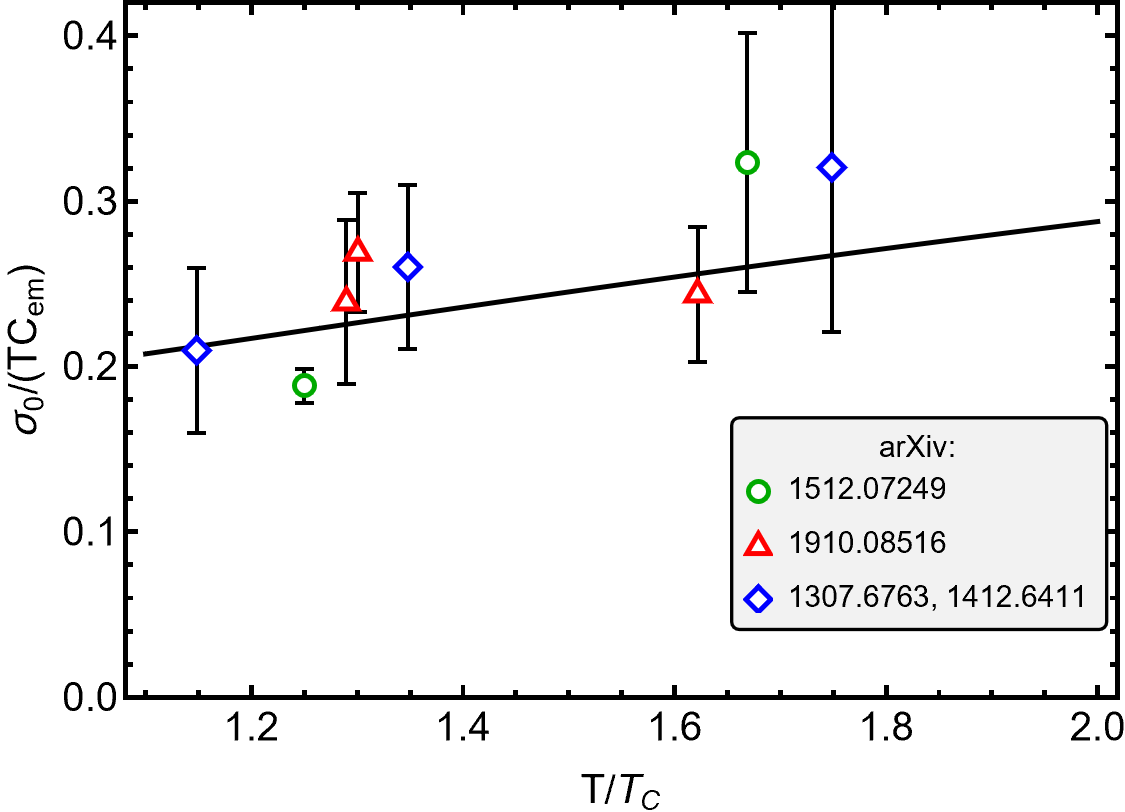
\includegraphics[width=0.75\linewidth]{plots/condcomp.png}
    \caption{The static conductivity $\sigma_0$ scaled with $T$ as a function of temperature $T$ scaled with the `critical' value $T_c\simeq 150\MeV$ as predicted by \req{eq:condstat}. `Experimental' data are lattice results adapted from \cite{Aarts:2020dda} for $T>T_c$.  We indicate each set of points by its arXiv reference: blue diamonds \cite{Amato:2013naa,Aarts:2014nba}, green circles \cite{Brandt:2015aqk}, and red triangles \cite{Astrakhantsev:2019zkr}. \radapt{Grayson:2024okq}.}
    \label{fig:lattice comp}
\end{figure}
%%%%%%%%%%%%%%%%%%%%%%%%%%%%

The  lattice-QCD results seen in  \rf{fig:lattice comp} \cite{Amato:2013naa,Aarts:2014nba,Brandt:2015aqk,Astrakhantsev:2019zkr} are scaled with temperature $T$ to remove the linear temperature dependence. One can see that the conductivity value predicted by \req{eq:kappadef}, plotted in \rf{fig:lattice comp} as a black line, lies well within the lattice-QCD results. We will use the value predicted by \rf{fig:lattice comp}, $\sigma = 5.01\,$MeV at $T=300\,$GeV, in the next section to compute the screened heavy-ion fields\index{heavy-ion!fields} in QGP.

One of the important situations to note in context of highly relativistic heavy-ion collisions  is that the fields of the ions, traveling near the speed of light, probe the polarization tensor, see \rsec{chap:PlasmaSF}, \req{eq:sigmaperp}, near the light cone. The transverse light-cone conductivity is given by
\begin{equation}\label{eq:lightcone}
    \sigma_\perp (\omega = |\boldsymbol{k}|)  =  i \frac{m_D^2}{4 \omega}\left( \frac{\kappa^2}{\omega^2} \xi \ln\xi +\frac{i\kappa}{\omega}\left(\xi+1\right)\right)\,,
\end{equation}
where $\xi$ is defined as
\begin{equation}\label{eq:xidef}
    \xi \equiv 1- 2i \frac{\omega}{\kappa}\,.
\end{equation}

%%%%%%%%%%%%%%%%%%%
%\label{sec:Maxwell2}
\para{Magnetic field in QGP during a nuclear collision}
Assuming that the QGP is an infinite homogeneous and stationary medium near equilibrium, we can solve Maxwell's equations for the self-consistent fields, see \rsec{sec:Maxwell}. Then the magnetic field\index{QGP!magnetic fields} is obtained by  Fourier transforming the momentum space expressions given in \reqs{eq:aperp}{eq:ftfields} to the position space
\begin{equation}\label{eq:magorgin}
   \boldsymbol{B}(t, z) = \int \frac{d^4k}{(2\pi)^4}  e^{-i\omega t+ik_z z}
 \frac{\mu_0 i \boldsymbol{k} \times\ft{j}_{\perp \text{ext}}(\omega, \boldsymbol{k})}{\boldsymbol{k}^2 - \omega^2 - \mu_0 \Pi_{\perp}(\omega, \boldsymbol{k})}\,.
\end{equation}
We choose the collision center as the origin of our spatial coordinate system and align the spatial $z$-axis with the beam direction. Due to the symmetry of the colliding ions, the only nonzero component of the magnetic field along the $z$-axis points out of the collision plane ($x-y$ plane). In our coordinate system used in \cite{Grayson:2022asf}, this corresponds to the $y$-component of the magnetic field. 

For ease of calculation, we specify the external 4-current using two colliding Gaussian charge distributions normalized to the nuclear root mean square radius $R$ and charge $Z$:
\begin{equation}\label{eq:rhoext}
\rho_{\text{ext}\pm }(t,\boldsymbol{x}) = \frac{Zq\gamma}{\pi^{3/2}R^3}e^{-\frac{1}{R^2}(x\mp b/2)^2}e^{-\frac{1}{R^2}y^2}
\times e^{-\frac{\gamma^2}{R^2}(z\mp \beta t)^2}\,,
\end{equation}
where $\gamma$ is  as before the Lorentz-factor, $\beta\to 1$ is the ratio of the ion speed to the speed of light, respectively, and $b$ is the impact parameter of the collision. The plus and minus signs indicate motion in the $\pm \hat{z}$-direction (beam-axis). This charge distribution corresponds to the vector current
\begin{equation}\label{eq:jext}
\boldsymbol{j}_{\text{ext}\pm}(t, \boldsymbol{x}) = \pm \beta \hatv{z} \rho_{\text{ext}\pm}(t, \boldsymbol{x})\,.
\end{equation}
Further details of the external charge distribution for two colliding nuclei are presented in Appendix B  of Ref.\,\cite{Grayson:2022asf}.

The numerical result for the position-space magnetic field found by Fourier transforming \req{eq:magorgin} using the full transverse polarization function \req{eq:polfuncsUltra} is shown as a red dashed line in \rf{fig:bfcomp} and compared with various models of conductivity. These other models and their connections to published works are discussed in detail in  Ref.\,\cite{Grayson:2022asf}.

%\phantom{Phantom text}
%%%%%%%%%%%%%%%%%%%%%%%%%%%%%
\begin{figure}
%\centering              
%\hspace{-0.04\linewidth}
%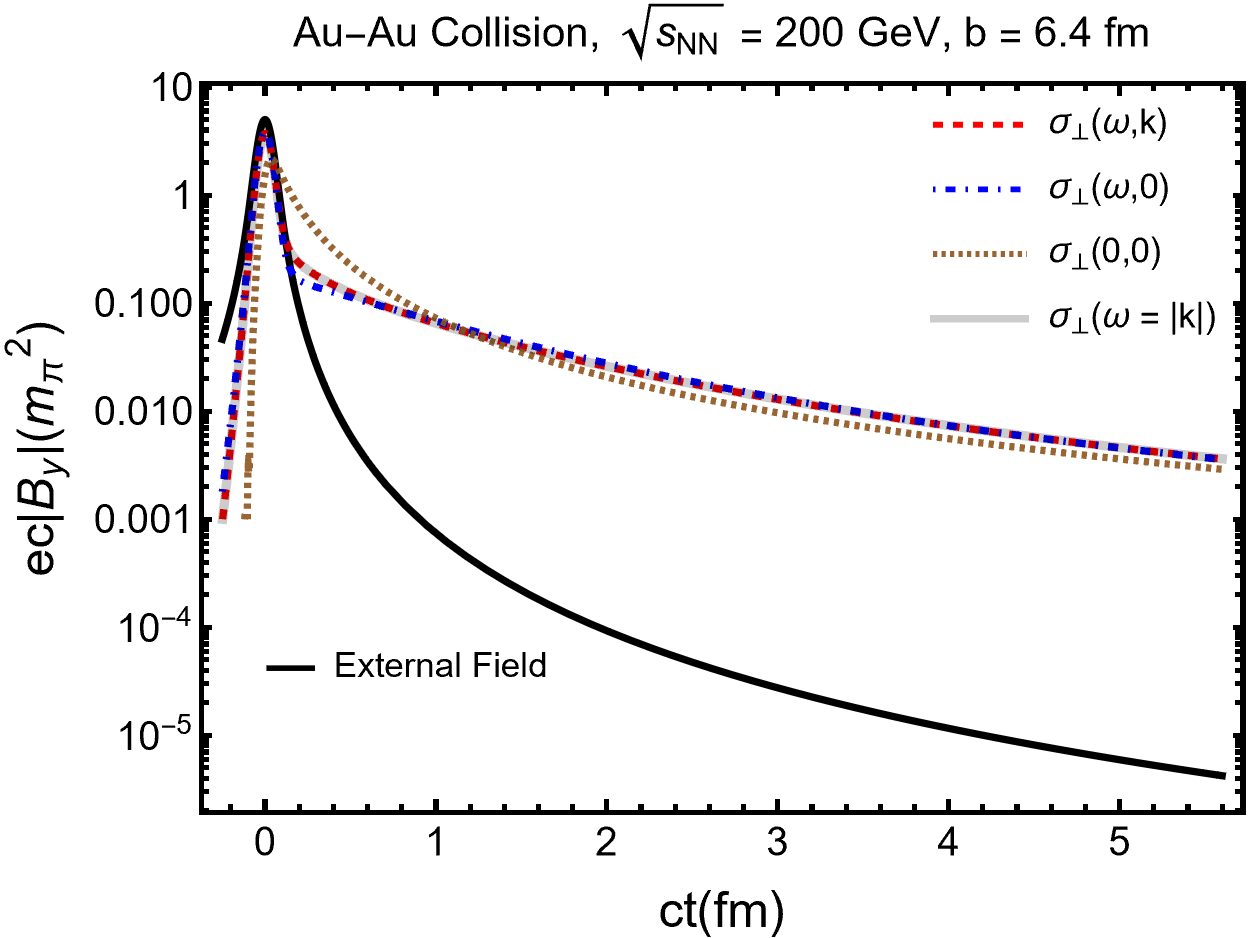
\includegraphics[width=0.955\linewidth]{plots/bf100.png}\\[0.4cm]
%%}
%%\includegraphics[width=0.89\linewidth]%{plots/bf100lin.png}
%%}
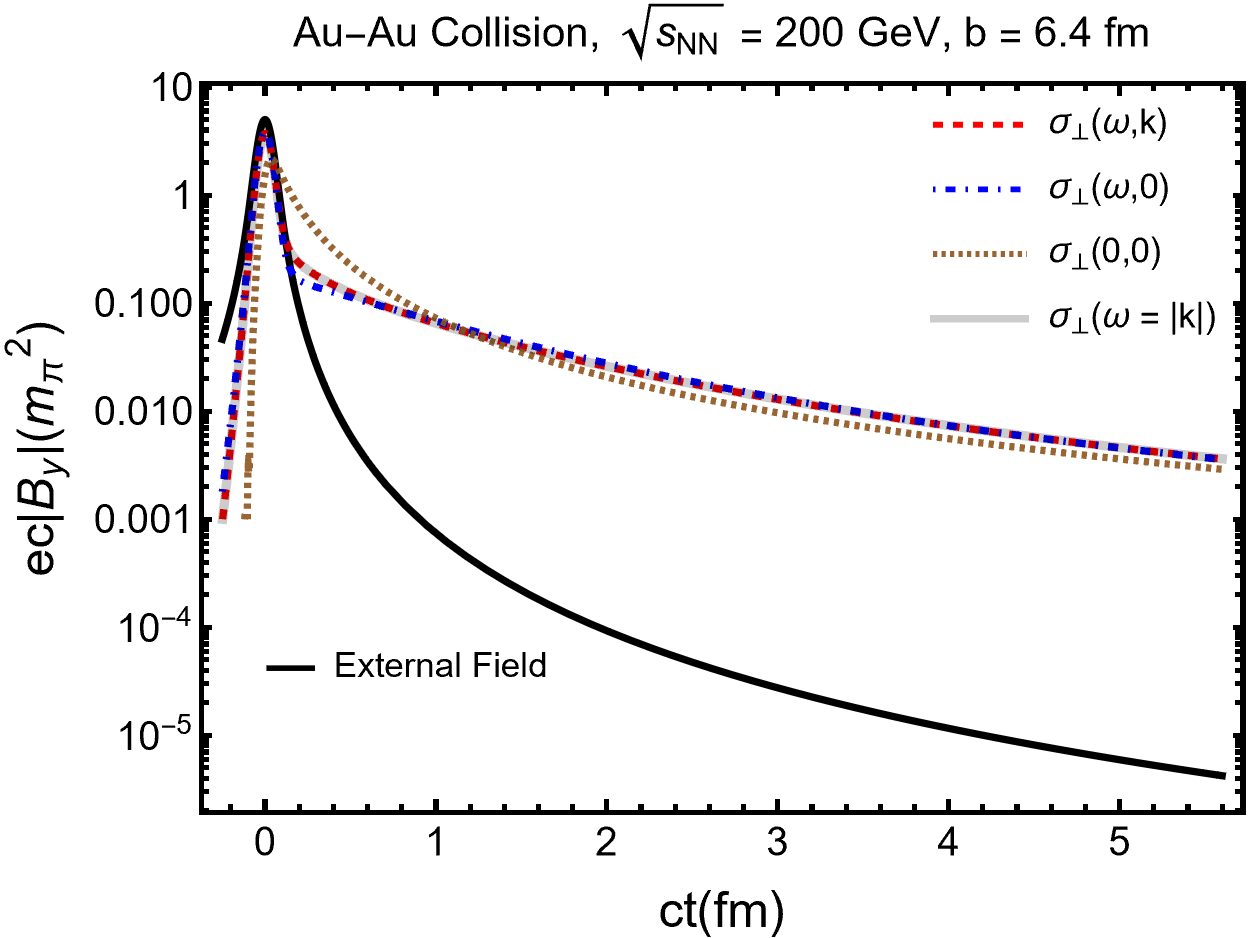
\includegraphics[width=0.50\linewidth]{plots/bf100.png}
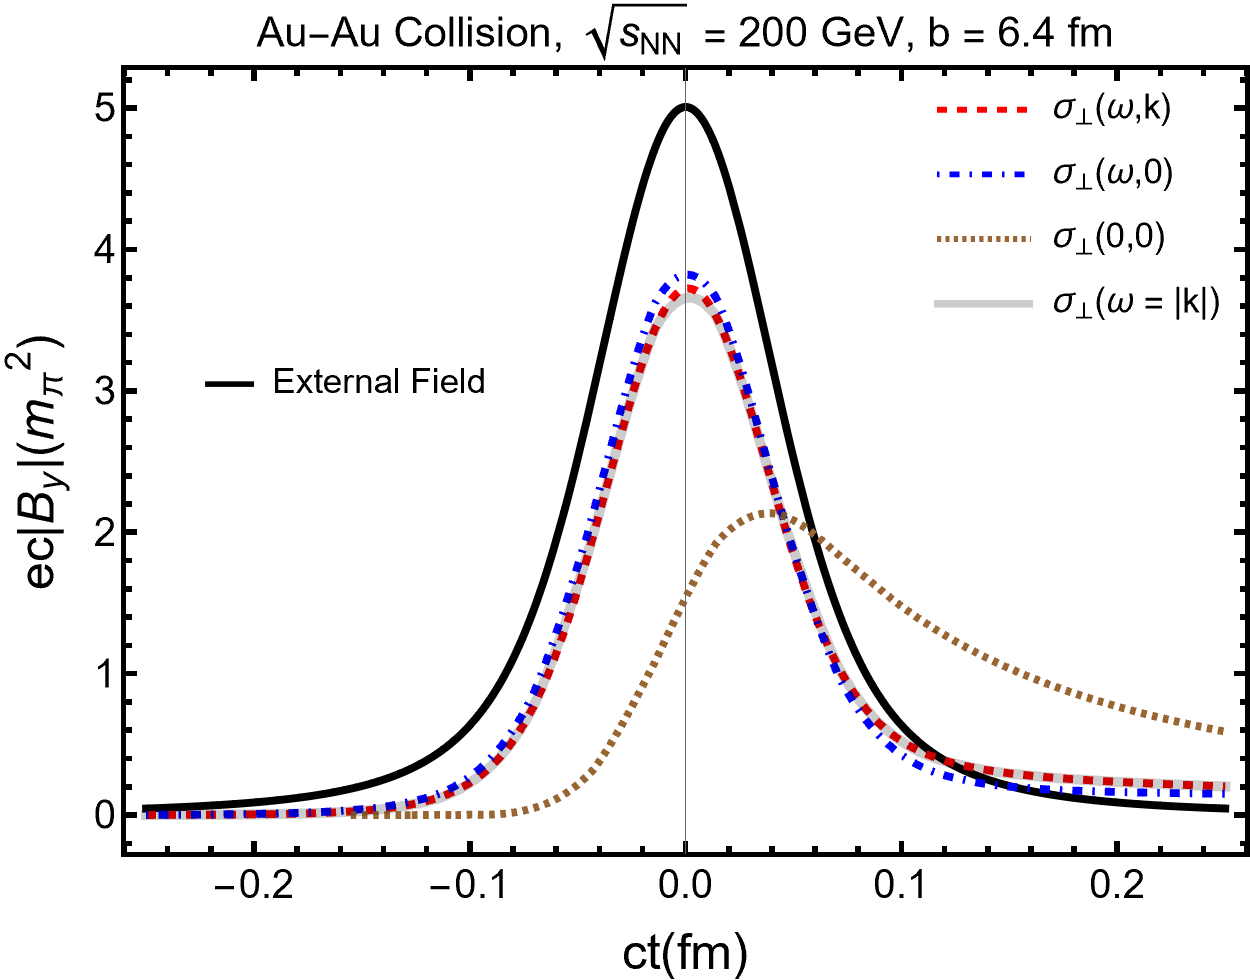
\includegraphics[width=0.47\linewidth]{plots/bf100lin.png}
\caption{The magnetic field at the collision center as a function of time, for QGP at $T = 300$\,MeV formed in Au-Au collisions ($Z=79$) at $\sqrt{s_\text{NN}} = 200$\,GeV and impact parameter $b = 6.4\,$fm. The left-hand frame shows the magnetic field\index{QGP!magnetic field} on a semi-logarithmic scale up to $ct = 5$\,fm. The right-hand frame shows the early-time magnetic field on a linear scale. \cccite{Grayson:2022asf}\label{fig:bfcomp}}
\end{figure}
%%%%%%%%%%%%%%%%%%%%%%%%%%%%%%% 

Note that the QGP plasma considered in \rf{fig:bfcomp} is homogeneous and stationary. In a more realistic situation, the field would become screened only after the QGP is formed in the collision. At the considered temperature $T = 300$\,MeV, the electromagnetic Debye mass is $m_D = 74\,$MeV, and the quark damping rate is $\kappa = 4.86\,m_D$. This gives a static conductivity of $\sigma_0 = 5.01\,$MeV. 

Comparing the different approximations   \rf{fig:bfcomp}, we see  all three approximations using static conductivity $\sigma_\bot(0,0)$, \req{eq:condstat}, the Drude conductivity $\sigma_\bot(\omega,0)$, \req{eq:drude},  and the light-cone conductivity $\sigma_\bot(\omega=\|\boldsymbol{k}|)$, \req{eq:lightcone},  have similar asymptotic behavior for large times and agree in outcome with the full conductivity $\sigma_\perp(\omega,\boldsymbol{k})$. However, the static conductivity fails to describe the field at the early times as seen very clearly in the right-hand frame of \rf{fig:bfcomp}. One subject of future study of the heavy-ion experimental environment is to use the light-cone conductivity to attain analytical formulas for electromagnetic fields in position space in light-cone coordinates.

The light-cone conductivity \req{eq:lightcone} simplifies the calculation of plasma response since it only depends on a single variable ($\omega = |\boldsymbol{k}|$). One can see in the right-hand frame of \rf{fig:bfcomp} that results obtained using the light-cone conductivity,\req{eq:lightcone}, shown as an opaque (grey) line, is hardly visible under the  dashed (red) line showing the full numerical solution \req{eq:magorgin}. The light-cone conductivity accurately models the early magnetic field in QGP formed in ion collisions since the ions traveling near the light's speed only sample the polarization tensor near the light-cone. 

The simplest method to calculate the late-time magnetic field of colliding nuclei is to assume a static conductivity \cite{Tuchin:2013apa}. In this case, the magnetic field\index{heavy-ion!magnetic fields} in Fourier space has the form
\begin{equation}\label{eq:bstat}
    \ft{B}(\omega,\boldsymbol{k}) = \frac{ \mu_0 i\boldsymbol{k} \times \ft{j}_{\perp \text{ext}}}{\boldsymbol{k}^2 - \omega^2 - i\omega\sigma_0}\,,
\end{equation}
which is Fourier transformed using contour integration in the appendix of \cite{Grayson:2022asf} to
\begin{equation}\label{eq:banalyticapp}
   B_y(t) = -\mu_0 \frac{ Zq \beta }{(2\pi)} \frac{ b\sigma_0}{4t^2} e^{\frac{-b^2 \sigma_0}{16 t}}\,.
\end{equation}

Looking at the left-hand frame of \rf{fig:bfcomp}, the static conductivity, dotted line, initially overestimates the magnetic field after the external field begins to disappear since the effect of dynamic screening is not captured. Approaching the freeze-out time $t_f \approx 5\,$fm/c every model of the response function predicts similar values for the magnetic field \cite{Song:2007ux}. This is because the static conductivity determines the dependence of the magnetic field at times later than $t>1/\sigma \approx 59$\,fm/c after which damping of the initial magnetic field pulse is irrelevant. 

Alternatively, by assuming a point-like charge distribution $R\rightarrow 0$ and approximating the magnetic field for $ 1/\sigma_0 > t\gg 1/\kappa$, one can derive the late-time magnetic field using the Drude conductivity \req{eq:drude}
\begin{equation}\label{eq:latetimeB}
   B_y(t) \approx  \mu_0 \frac{ Ze \beta b \kappa \omega_p }{8\pi}\bigg[ \frac{1- e^{-\kappa t}}{\kappa t} - e^{-\kappa t} \text{Ei}\left(t\kappa\right)\bigg]\,.
\end{equation}
This result has the advantage of accurately describing the late-time magnetic field $t>t_f$  at large $\gamma$ as shown in \rf{fig:bcolcomp}. Both these results illustrate that the late-time magnetic field has a finite limit when $\gamma\rightarrow\infty$ as it depends only on $\beta\to 1$, but not on $\gamma$. The approximation used to derive this solution holds for $\gamma\beta \gg \sqrt{ \kappa/\sigma_0} \approx 12$. 

%%%%%%%%%%%%%%%%%%%%%%%%
\begin{figure}
\centering
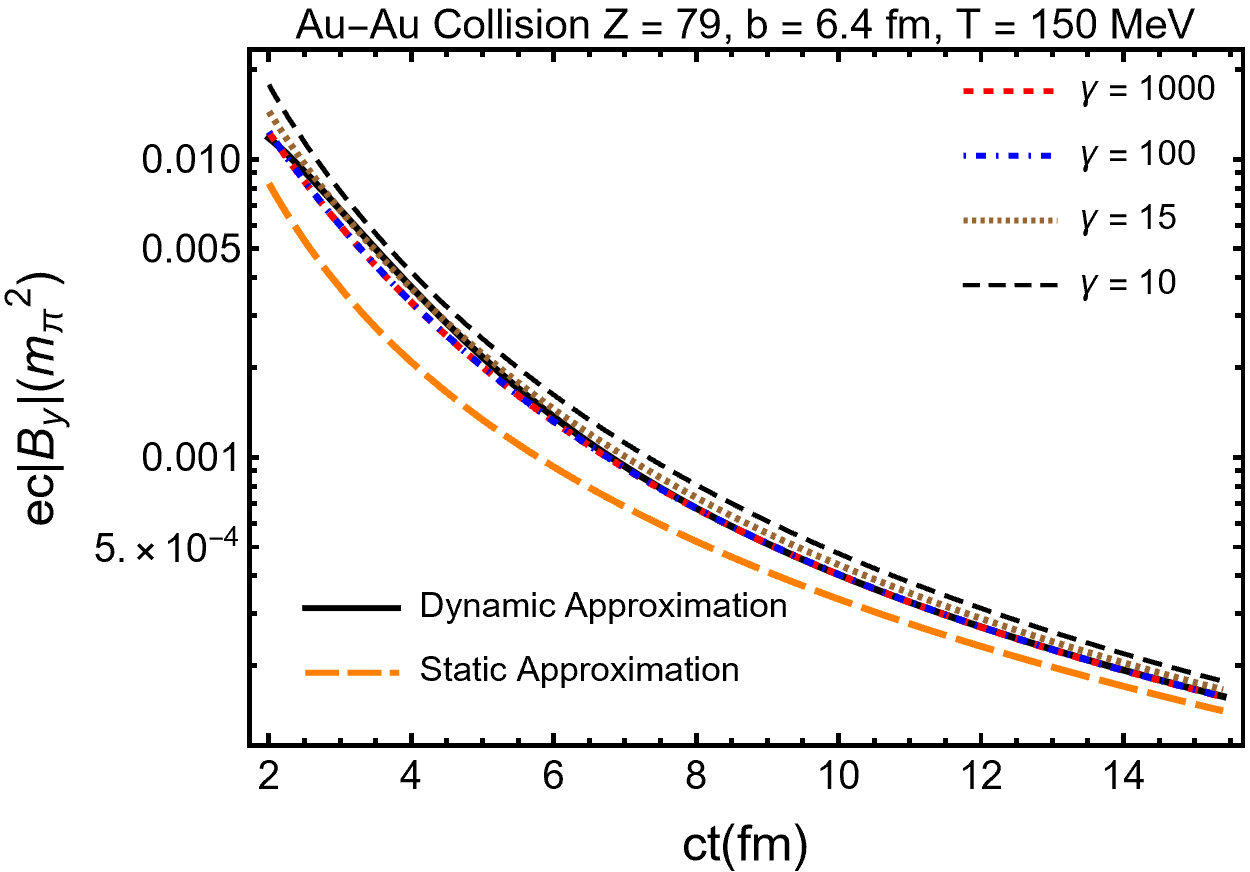
\includegraphics[width=0.8\linewidth]{plots/bfgaamacomp.png}
    \caption{The freeze-out magnetic field for $T= 150$\,MeV for collisions with colliding heavy-ions at different value of Lorentz-factor, $\gamma=10,15,100,1000$ as function of freeze-out time.   \radapt{Grayson:2022asf}\label{fig:bcolcomp}}
\end{figure}
%%%%%%%%%%%%%%%%%%%%%%

In \rf{fig:bcolcomp} we study the freeze-out magnetic field for $T= 150$\,MeV for collisions with colliding heavy-ions. We expect that around this temperature, QGP will hadronize \cite{Letessier:1992xd}.  We compare \req{eq:banalyticapp} to the full numerical result using the full polarization tensor \req{eq:magorgin} and explore dependence on the Lorentz-factor $\gamma\in\{10,1000\}$. The approximate static late time solution \req{eq:banalyticapp} shown as an orange dashed line is compared to numerical calculations  and to the late time analytic expansion \req{eq:latetimeB}. The approximate solution does not fully match the ultrarelativistic limit until times $t > t_{\sigma} \approx 59$\,fm/c. The freeze-out magnetic field\index{freeze-out!magnetic field} at fixed freeze-out time and temperature $T= 150$\,MeV \req{eq:banalyticapp} (black solid line) is independent of the beam energy over a wide range of $\gamma$. It begins to diverge slowly from the ultra-relativistic case at around $\gamma \leq 15$ for the time window shown in the figure. Lower beam energies result in a somewhat larger field at late times.  

As seen in \rf{fig:bcolcomp} the late-time magnetic field has a very soft dependence on the heavy-ion collision energy. However, the time $t_f$ at which QGP hadronization\index{QGP!hadronization} occurs, varies with collision energy; this has a much stronger effect on the magnitude of the freeze-out field.  As the QGP begins to hadronize at time $t_f$, one may expect hadrons to be statistically polarized with respect to the magnetic field. In \cite{Muller:2018ibh} the measured difference in global polarization of hyperons\index{hyperon!polarization} and anti-hyperons is used to give an upper bound on the magnetic field at QGP freeze-out, $B \sim 2.7\times 10^{-3}\,m_{\pi}^2$ for Au+Au collisions at $\sqrt{s_\text{NN}} = 200$\,GeV. Looking at \rf{fig:bcolcomp} the magnetic field for $\gamma = 100$ at QGP freeze-out $t_f \approx 5 $\,fm/c is predicted to be $B \approx 1.2\times 10^{-3}\,m_{\pi}^2$, somewhat below this upper bound. Note that this assumes the polarization rapidly equilibrates in the plasma. It also neglects any interactions during the hadron gas stage\index{hadrons gas}  of the collision. 

Since the remnant magnetic field at hadronization does not depend directly on the collision energy, an experimental measurement of the magnetic field at different collision energies could permit the determination of the electrical conductivity of the QGP or a determination of the freeze-out time of QGP if the conductivity is assumed to be known. As discussed at the beginning we are particularly interested in the primordial cosmic QGP conductivity which allows us to model the response of primordial plasma to strong magnetic fields. 
